%%%%%%%%%%%%%%%%%%%%%%%%%%%%%%%%%%%%%%%%%%%%%%%%%%%%%%%%%%%%%%%%%%%%%%%%%%%%%%
%%
%%
%%  奈良工業高等専門学校 情報工学科
%%
%%  第 4 学年 コンピュータ援用論理設計
%%
%%        「8bitCPUの組み合わせ回路」実験報告書
%%
%%                作成日 平成 28 年  6 月 24 日 金(PDFpLaTeX 版)
%%                提出日 平成 28 年  6 月 24 日 金(PDFpLaTeX 版)
%%
%%            池内隆一郎 (an94_49@yahoo.co.jp)
%%
%%
%%%%%%%%%%%%%%%%%%%%%%%%%%%%%%%%%%%%%%%%%%%%%%%%%%%%%%%%%%%%%%%%%%%%%%%%%%%%%%

\documentclass[12pt]{jreport}

\setlength{\topmargin}{-12.5truemm}
\usepackage{here}
\setlength{\textheight}{\paperheight}   % 紙面縦幅を本文領域にする(BOTTOM=-TOP)
\setlength{\topmargin}{-5.4truemm}      % 上の余白を20mm(=1inch-5.4mm)に
\addtolength{\topmargin}{-\headheight}  % 
\addtolength{\topmargin}{-\headsep}     % ヘッダの分だけ本文領域を移動させる
\addtolength{\textheight}{-50truemm}    % 下の余白は30mm(BOTTOM=-TOPだから+TOP+30mm)
\setlength{\textwidth}{\paperwidth}     % 紙面横幅を本文領域にする(RIGHT=-LEFT)
\setlength{\oddsidemargin}{-5.4truemm}  % 左の余白を20mm(=1inch-5.4mm)に
\setlength{\evensidemargin}{-5.4truemm} % 
\addtolength{\textwidth}{-40truemm}     % 右の余白も20mm(RIGHT=-LEFT)

% \usepackage[dviout]{graphicx}
\usepackage{comment}    % comment 環境を使うためのスタイルファイル

\usepackage{listings}

%
%    ↓丸みのある四角や影付きの四角などを使うためのスタイルファイル
%
\usepackage{fancybox}    % shadowbox, ovalbox 環境を使うためのスタイルファイル
\usepackage{ascmac}    % screen 環境を使うためのスタイルファイル
\usepackage{framed}    % framed 環境を使うためのスタイルファイル

%
%    ↓PostScript 形式 や EPS 形式の図を張り付けるためのスタイルファイル
%
\usepackage{float}    % 図や表を記述した位置に置くためのスタイルファイル
\usepackage[dvipdfmx]{graphicx}    % 回転などもできるスタイルファイル

%
%    箇条書きに関するスタイルファイル
%
\usepackage{enumitem}    % 拡張 enumerate 環境を使うためのスタイルファイル

\makeatother
\title{コンピュータ援用論理設計中間課題 \vspace{5cm}}
\author{\hspace{10cm} 4 年 情報工学科 2番 \\\\\hspace{9cm} 提出者: 4班 池内 隆一郎}
\date{\vspace{5cm}\hspace{-10cm}提出締め切り: 平成28年6月24日(金)\\\hspace{-115mm} 提出日: 平成28年 6月24日(金)\\\hspace{-143mm}}


\begin{document}
    
    \maketitle
    \newpage

    \chapter*{第1章 課題内容}
         課題内容は, 以下に指定する8bitのCPUを作成し考察することである.  CPUの仕様について表1にCPUの命令表を示す. この仕様通りに8bitCPUの内部には, ALU, デコーダ, マルチプレクサ1, マルチプレクサ2を作成しそれを一つの回路にまとめ, テストを行い正しく動作しているか確認する. 最終的な入出力仕様は以下の通りである. 
         
         \subsection*{\ \ 入力}
            \begin{itemize}
                \item Ain, Bin, Cin, Din (8bit) : 各レジスタの出力から与えられる入力
                \item Carryin (1bit) : Carryフラグから与えられる入力
                \item op (4bit) : プログラムカウンタから与えられる機械語
            \end{itemize}
         \subsection*{\ \ 出力}
            \begin{itemize}
                \item Aout, Bout, Cout, Dout (8bit) : 各レジスタへの出力
                \item Carryout (1bit) : 加算器の桁上げの有無
            \end{itemize}

            \begin{table}[htb]
              \begin{center}
                \caption{CPU命令表}
                \begin{tabular} {|c|c|l||l|} \hline
                  機械語 & 命令 & op & ニーモック \\ \hline \hline
                  0000 & ADD & A, B & A \verb|<|= A + B \\ \hline
                  0001 & ADC & A, B & A \verb|<|= A + B + Carry \\ \hline
                  0010 & SUB & A, B & A \verb|<|= A - B \\ \hline
                  0011 & MUL & A, B & A \verb|<|= A * B \\ \hline

                  0100 & AND & A, B & A \verb|<|= A and B \\ \hline
                  0101 & OR & A, B & A \verb|<|= A or B \\ \hline
                  0110 & NOT & A & A \verb|<|= not A \\ \hline
                  0111 & XOR & A, B & A \verb|<|= A xor B \\ \hline

                  1000 & LD & A, B & A \verb|<|= B \\ \hline
                  1001 & LD & A, C & A \verb|<|= C \\ \hline
                  1010 & LD & A, D & A \verb|<|= D \\ \hline
                  1011 & LD & B, A & B \verb|<|= A \\ \hline

                  1100 & LD & B, C & B \verb|<|= C \\ \hline
                  1101 & LD & B, D & B \verb|<|= D \\ \hline
                  1110 & LD & C, A & C \verb|<|= A \\ \hline
                  1111 & LD & D, A & D \verb|<|= A \\ \hline
                \end{tabular}
              \end{center}
            \end{table}

    \chapter*{第2章 ALU}
        ALUのverilogモジュールとテストのソースコード, alu\_p44.v, alu\_44\_tb.vと, 実行結果のタイミングチャートをソースコード1, ソースコード2, 図1に示す. 

        \begin{center}
            \begin{lstlisting}[basicstyle=\ttfamily\footnotesize, frame=single]
module alu_pp44(Ain, Bin, Carryin, op, alu_enabled, Carryout, alu_out);
   input [7:0] Ain, Bin;
   input Carryin;
   input [2:0] op;
   input alu_enabled;
   output Carryout;
   output [7:0] alu_out;

   function [7:0] operate;
      input [7:0] Ain;
      input [7:0] Bin;
      input [2:0] op;
      input Carryin;
      input alu_enabled;
      begin
         if (alu_enabled == 1) begin
            case(op)
               3'b000: operate = Ain + Bin;
               3'b001: operate = Ain + Bin + Carryin;
               3'b010: operate = Ain - Bin;
               3'b011: operate = Ain * Bin;
               3'b100: operate = Ain & Bin;
               3'b101: operate = Ain | Bin;
               3'b110: operate = ~Ain;
               3'b111: operate = Ain ^ Bin;
            endcase
         end else operate = Ain;
      end
   endfunction
   function carry;
      input [7:0] Ain;
      input [7:0] Bin;
      input Carryin;
      input [2:0] op;
      begin
         if (alu_enabled == 1 && op == 3'b001) carry = (Ain + Bin
            + Carryin > 8'h80) ? 0 : 1;
      end
   endfunction
   assign alu_out = operate(Ain, Bin, op, Carryin, alu_enabled);
   assign Carryout = carry(Ain, Bin, Carryin, op);
endmodule
            \end{lstlisting}
            ソースコード1 alu\_pp44.v
        \end{center}



        \begin{center}
            \begin{lstlisting}[basicstyle=\ttfamily\footnotesize, frame=single]
module alu_pp44_tb;

    // Inputs
    reg [7:0] Ain;
    reg [7:0] Bin;
    reg Carryin;
    reg [2:0] op;
    reg alu_enabled;

    // Outputs
    wire Carryout;
    wire [7:0] alu_out;

    // Instantiate the Unit Under Test (UUT)
    alu_pp44 uut (
        .Ain(Ain), 
        .Bin(Bin), 
        .Carryin(Carryin), 
        .op(op), 
        .alu_enabled(alu_enabled), 
        .Carryout(Carryout), 
        .alu_out(alu_out)
    );

    initial begin
        // Initialize Inputs
        Ain = 0;
        Bin = 0;
        Carryin = 0;
        op = 0;
        alu_enabled = 0;

        // Wait 100 ns for global reset to finish
        #20 Ain = 25;  Bin = 145; Carryin = 0; op = 6; alu_enabled = 0;

        #20 Ain = 251; Bin = 203; Carryin = 0; op = 0; alu_enabled = 1;
        #20 Ain = 21;  Bin = 45;  Carryin = 1; op = 0; alu_enabled = 1;
        #20 Ain = 248; Bin = 146; Carryin = 0; op = 0; alu_enabled = 1;

        #20 Ain = 31;  Bin = 96;  Carryin = 1; op = 1; alu_enabled = 1;
        #20 Ain = 57;  Bin = 211; Carryin = 1; op = 1; alu_enabled = 1;
        #20 Ain = 78;  Bin = 160; Carryin = 0; op = 1; alu_enabled = 1;

        #20 Ain = 13;  Bin = 24;  Carryin = 0; op = 2; alu_enabled = 1;
        #20 Ain = 189; Bin = 50;  Carryin = 1; op = 2; alu_enabled = 1;
        #20 Ain = 123; Bin = 26;  Carryin = 0; op = 2; alu_enabled = 1;

        #20 Ain = 117; Bin = 108; Carryin = 1; op = 3; alu_enabled = 1;
        #20 Ain = 126; Bin = 4;   Carryin = 0; op = 3; alu_enabled = 1;
        #20 Ain = 39;  Bin = 226; Carryin = 0; op = 3; alu_enabled = 1;

        #20 Ain = 243; Bin = 87;  Carryin = 0; op = 4; alu_enabled = 1;
        #20 Ain = 84;  Bin = 16;  Carryin = 1; op = 4; alu_enabled = 1;
        #20 Ain = 156; Bin = 53;  Carryin = 1; op = 4; alu_enabled = 1;

        #20 Ain = 222; Bin = 237; Carryin = 0; op = 5; alu_enabled = 1;
        #20 Ain = 98;  Bin = 44;  Carryin = 1; op = 5; alu_enabled = 1;
        #20 Ain = 190; Bin = 24;  Carryin = 1; op = 5; alu_enabled = 1;

        #20 Ain = 55;  Bin = 200; Carryin = 0; op = 6; alu_enabled = 1;
        #20 Ain = 186; Bin = 32;  Carryin = 1; op = 6; alu_enabled = 1;
        #20 Ain = 101; Bin = 57;  Carryin = 1; op = 6; alu_enabled = 1;

        #20 Ain = 252; Bin = 234; Carryin = 0; op = 7; alu_enabled = 1;
        #20 Ain = 11;  Bin = 107; Carryin = 1; op = 7; alu_enabled = 1;
        #20 Ain = 188; Bin = 230; Carryin = 0; op = 7; alu_enabled = 1;

        #20 $finish;
    end
endmodule

            \end{lstlisting}
            ソースコード2 alu\_pp44\_tb.v \\ \\
        \end{center}

        \begin{center}
            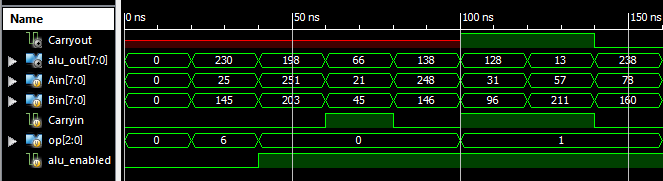
\includegraphics[width=18cm]{apu_op44_1.png} \\ \\
            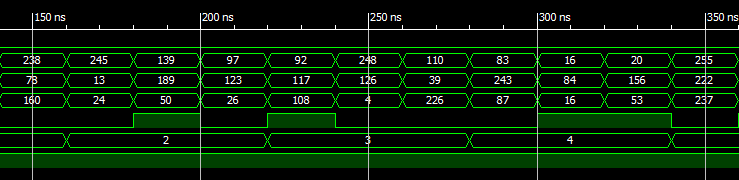
\includegraphics[width=18cm]{apu_op44_2.png} \\ \\
            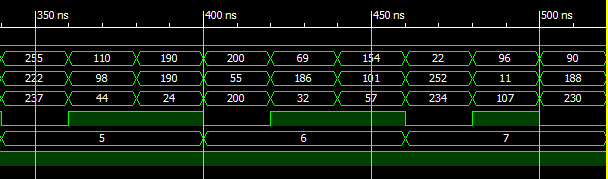
\includegraphics[width=18cm]{apu_op44_3.png} \\ \\
                図1 alu\_pp44のタイミングチャート
        \end{center}

        図1の実行結果をまとめ, ALUの実行結果の入出力表を3に示す. 

        \begin{table}[htb]
          \begin{center}
            \caption{alu\_p44の入出力表}
            \begin{tabular} {|c|c|c|c|c|c|c|} \hline
                \multicolumn{5}{|c|}{入力} & \multicolumn{2}{|c|}{出力} \\ \hline \hline
                Ain & Bin & Carryin & op & alu\_enabled & alu\_out & Carryout \\ \hline
                25 & 145 & 0 & 6 & 0 & 230 & 不定 \\ \hline
                251 & 203 & 0 & 0 & 1 & 198 & 不定 \\ \hline
                21 & 45 & 1 & 0 & 1 & 66 & 不定 \\ \hline
                248 & 146 & 0 & 0 & 1 & 138 & 不定 \\ \hline
                31 & 96 & 1 & 1 & 1 & 128  & 1 \\ \hline
                57 & 211 & 1 & 1 & 1 & 13 & 1 \\ \hline
                78 & 160 & 0 & 1 & 1 & 238 & 0 \\ \hline
                13 & 24 & 0 & 2 & 1 & 245 & 0 \\ \hline
                189 & 50 & 1 & 2 & 1 & 139 & 0 \\ \hline
                123 & 26 & 0 & 2 & 1 & 97 & 0 \\ \hline
                117 & 108 & 1 & 3 & 1 & 92 & 0 \\ \hline
                126 & 4 &  0 & 3 & 1 & 248 & 0 \\ \hline
                39 & 226 & 0 & 3 & 1 & 110 & 0 \\ \hline
                243 & 87 & 0 & 4 & 1 & 83 & 0 \\ \hline
                84 & 16 & 1 & 4 & 1 & 16 & 0 \\ \hline
                156 & 53 & 1 & 4 & 1 & 20 & 0 \\ \hline
                222 & 237 & 0 & 5 & 1 & 255 & 0 \\ \hline
                98 & 44 & 1 & 5 & 1 & 110 & 0 \\ \hline
                190 & 24 & 1 & 5 & 1 & 190 & 0 \\ \hline
                55 & 200 & 0 & 6 & 1 & 200 & 0 \\ \hline
                186 & 32 & 1 & 6 & 1 & 69 & 0 \\ \hline
                101 & 57 & 1 & 6 & 1 & 154 & 0 \\ \hline
                252 & 234 & 0 & 7 & 1 & 22 & 0 \\ \hline
                11 & 107 & 1 & 7 & 1 & 96 & 0 \\ \hline
                188 & 230 & 0 & 7 & 1 & 90 & 0 \\ \hline
            \end{tabular}
          \end{center}
        \end{table}


        ソースコード1, 2, 図1, 表2について, alu\_enabled端子とALUが正しく動作していることについて説明する. 
        \begin{itemize}
            \item alu\_enabled端子: 全体の回路で1章の表1の命令表の機械語1001が入力された場合, ALUのopselには001が入力される. ここでもしalu\_enabled端子がなければ, Carryoutを書き換えてしまい前の値を正常に受け継げない. 機械語0001と1001を判別するために, ソースコード1のようにalu\_enabled端子を作成しこれにより, Carryout端子が正常に前の値をそのまま使うように設計した. また, これにより, ALUを使わない場合(LD命令を使う場合)に複雑なcase文を通らなくて済むので, 性能の向上を期待することができる.  \newpage

            \item ALUが正しく動作しているか: 表2の実行結果より, 以下の式が成り立つので出力が正しいということが確認できる. また, Carryoutは前の値を正しく受け継いでいるのでALUは正しく動作している. 
            \begin{eqnarray*}
                alu\_out &=& 25 = \overline{00011001} = 11100110 = 230\\
                alu\_out &=& 251 + 203 = 11111011 + 11001011 = \left(1\right)11000110 = 198\\
                alu\_out &=& 21 + 45 = 66\\    
                alu\_out &=& 248 + 146 = 11111000 + 10010010 = \left(1\right)10001010 = 138\\
                alu\_out &=& 31 + 96 + 1 == 128\\
                alu\_out &=& 57 + 211 = 111001 + 11010011 = 00001100 = 100001100 = 12\\
                alu\_out &=& 78 + 160 = 238\\
                alu\_out &=& 13 - 24 = 100000000 - 00001011 = 11110101 = 245\\
                alu\_out &=& 189 - 50 = 139\\
                alu\_out &=& 123 - 26 = 97\\
                alu\_out &=& 117 * 108 = 1110101 * 1101100 = \left(11000\right)101011100 = 92\\
                alu\_out &=& 126 * 4  = 1111110 * 100 = \left(1)\right)11111000 = 248\\
                alu\_out &=& 39 * 226 = 100111 * 11100010 = \left(10001)\right)001101110 = 110\\
                alu\_out &=& 243 and 87 = 11110011 \wedge 1010111 = 83\\
                alu\_out &=& 84 and 16 = 1010100 \wedge 10000 = 16\\
                alu\_out &=& 156 and 53 = 100111004 \wedge 110101 = 10100 = 20\\
                alu\_out &=& 222 or 237 = 11011110 \vee 11101101 = 11111111 = 255\\
                alu\_out &=& 98 or 44 = 1100010 \vee 101100 = 1101110 = 110\\
                alu\_out &=& 190 or 24 = 10111110 \vee 11000 = 10111110 = 190\\
                alu\_out &=& not 55 = \overline{110111} = 11001000 = 200\\
                alu\_out &=& not 186 = \overline{10111010} = 1000101 = 69\\
                alu\_out &=& not 101 = \overline{1100101} = 10011010 = 154\\
                alu\_out &=& 252 xor 234 = 11111100 \oplus 11101010 = 10110 = 22\\
                alu\_out &=& 1 xor 107 = 1 \oplus 1101011 = 1100000 = 96\\
                alu\_out &=& 188 xor 230 = 10111100 \oplus 11100110 = 1011010 = 90\\
            \end{eqnarray*}

        \end{itemize}

    \chapter*{第3章 デコーダ}
        デコーダのverilogモジュールとテストのソースコード, op\_decode.v, op\_decode\_tb.vと, 実行結果のタイミングチャートをソースコード3, ソースコード4, 図2に示す. 
        \begin{center}
            \begin{lstlisting}[basicstyle=\ttfamily\footnotesize, frame=single]
module op_decode(op, op_sel, reg_sel1, reg_sel2, alu_enabled);
    input[3:0] op;
    
    output[2:0] op_sel;
    output[1:0] reg_sel1, reg_sel2;
    output alu_enabled;
    
    reg[2:0] op_sel;
    reg[1:0] reg_sel1, reg_sel2;
    reg alu_enabled;
    
    always @(op) begin
        if (op < 4'b1000) begin
                op_sel <= op;
                reg_sel1 <= 2'b11;
                reg_sel2 <= 2'b10;
                alu_enabled <= 1;
        end else begin
            op_sel <= 0;
            alu_enabled <= 0;
            if (op < 4'b1011) reg_sel1 <= op;
            else begin
                reg_sel1 <= 2'b11;
                if (op < 4'b1110) reg_sel2 <= op;
                else reg_sel2 <= 2'b10;
            end
        end
    end
    
endmodule
            \end{lstlisting}
            ソースコード3 op\_decode.v
        \end{center}
        \newpage

        \begin{center}
            \begin{lstlisting}[basicstyle=\ttfamily\footnotesize, frame=single]

module op_decode_tb;

    // Inputs
    reg [3:0] op;

    // Outputs
    wire [2:0] op_sel;
    wire [1:0] reg_sel1;
    wire [1:0] reg_sel2;
    wire alu_enabled;

    // Instantiate the Unit Under Test (UUT)
    op_decode uut (
        .op(op), 
        .op_sel(op_sel), 
        .reg_sel1(reg_sel1), 
        .reg_sel2(reg_sel2), 
        .alu_enabled(alu_enabled)
    );

    initial begin
        // Initialize Inputs
        op = 0;

        // Wait 100 ns for global reset to finish
        #50 op = 4'b0000;
        #50 op = 4'b0001;
        #50 op = 4'b0010;
        #50 op = 4'b0011;

        #50 op = 4'b0100;
        #50 op = 4'b0101;
        #50 op = 4'b0110;
        #50 op = 4'b0111;

        #50 op = 4'b1000;
        #50 op = 4'b1001;
        #50 op = 4'b1010;
        #50 op = 4'b1011;

        #50 op = 4'b1100;
        #50 op = 4'b1101;
        #50 op = 4'b1110;
        #50 op = 4'b1111;

        #50 $finish;
        
        // Add stimulus here

    end
      
endmodule
            \end{lstlisting}
            ソースコード4 op\_decode\_tb.v
        \end{center}

        \begin{center}
            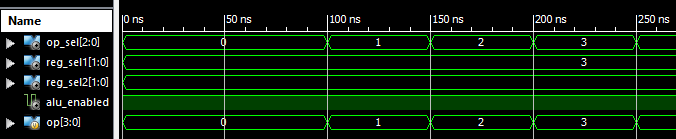
\includegraphics[width=18cm]{op_decode_1.png} \\ \\
            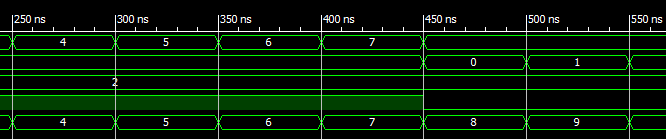
\includegraphics[width=18cm]{op_decode_2.png} \\ \\
            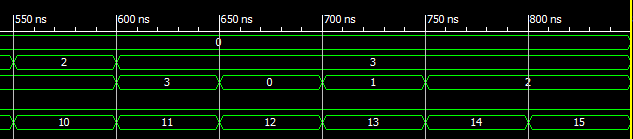
\includegraphics[width=18cm]{op_decode_3.png} \\ \\
                図2 op\_decodeのタイミングチャート
        \end{center} 
        \newpage

        図2の実行結果をまとめ, op\_decodeの実行結果の入出力表を表3に示す. 

        \begin{table}[htb]
          \begin{center}
            \caption{op\_decodeの入出力表}
            \begin{tabular} {|c|c|c|c|c|} \hline
              入力 & \multicolumn{4}{|c|}{出力} \\ \hline \hline
                op & op\_sel & reg\_sel1 & reg\_sel2 & alu\_enabled \\ \hline
                0000 & 0 & 3 & 2 & 1 \\ \hline
                0001 & 1 & 3 & 2 & 1 \\ \hline
                0010 & 2 & 3 & 2 & 1 \\ \hline
                0011 & 3 & 3 & 2 & 1 \\ \hline

                0100 & 4 & 3 & 2 & 1 \\ \hline
                0101 & 5 & 3 & 2 & 1 \\ \hline
                0110 & 6 & 3 & 2 & 1 \\ \hline
                0111 & 7 & 3 & 2 & 1 \\ \hline

                1000 & 0 & 0 & 2 & 0 \\ \hline
                1001 & 1 & 1 & 2 & 0 \\ \hline
                1010 & 2 & 2 & 2 & 0 \\ \hline
                1011 & 3 & 3 & 3 & 0 \\ \hline

                1100 & 4 & 3 & 0 & 0 \\ \hline
                1101 & 5 & 3 & 1 & 0 \\ \hline
                1110 & 6 & 3 & 2 & 0 \\ \hline
                1111 & 7 & 3 & 2 & 0 \\ \hline

            \end{tabular}
          \end{center}
        \end{table}


        ソースコード3, 4, 図2, 表3より, デコーダ(op\_decode)が正しく動作していることについて説明する. 
        第2章ALUで説明した通り, ALUを有効かするかどうかを判定しなければ, Carryoutが正しく動作しないため, alu\_enabled端子を出力端子として作成した. この端子は, 命令(op)の最上位bitが0から始まるのみ1を出力しALUを有効化する. op\_selには, 下位3bitを出力することにより, ALUにどの演算かを伝える. また, reg\_sel1, 2には, 不定を出力させないために各マルチプレクサーを使わない命令の場合は, そのままAin, Binを, Aout, Bout, へ出力できるようにした. マルチプレクサー4(reg\_sel1)では3, マルチプレクサー3(reg\_sel2)では2を出力することにより, 各マルチプレクサを使わない場合に入力をそのまま返すことができる. 転送命令(LD)の場合は 下位2bitを出力することによりどこから転送するかを決定する. 表2より命令(op)が上位1bitが1の場合は, 演算命令なのでalu\_enabled端子をHighにし, 下位3itをop\_selへ出力し, 命令(op)
        がマルチプレクサを使う場合は使うマルチプレクサにreg\_selに下位2bitを出力しているので, デコーダの実行結果は正しく動作していることが確認できる. 


    \chapter*{第4章 マルチプレクサー}
        マルチプレクサmux3, mux4のverilogモジュールとテストのソースコード, mux3.v, mux3\_tb.v, mux4.v, mux4\_tb.v, それぞれの実行結果のタイミングチャートをソースコード5, ソースコード6, ソースコード7, ソースコード8, 図3, 図4に示す. 
        \begin{center}
            \begin{lstlisting}[basicstyle=\ttfamily\footnotesize, frame=single]
module mux3(Ain, Bin, Cin, Din, reg_sel, Bout);
    input[7:0] Ain, Bin, Cin, Din;
    input[1:0] reg_sel;

    output[7:0] Bout;
    
    function [7:0] select;
        input [7:0] Ain, Bin, Cin, Din;
        input [1:0] reg_sel;
        begin
            case (reg_sel)
                2'b11: select = Ain;
                2'b00: select = Cin;
                2'b01: select = Din;
                2'b10: select = Bin;
            endcase
        end
    endfunction

    assign Bout = select(Ain, Bin, Cin, Din, reg_sel);
endmodule
            \end{lstlisting}
            ソースコード5 mux3.v
        \end{center}

        \begin{center}
            \begin{lstlisting}[basicstyle=\ttfamily\footnotesize, frame=single]
module mux3_tb;

    // Inputs
    reg [7:0] Ain;
    reg [7:0] Bin;
    reg [7:0] Cin;
    reg [7:0] Din;
    reg [1:0] reg_sel;

    // Outputs
    wire [7:0] Bout;

    // Instantiate the Unit Under Test (UUT)
    mux3 uut (
        .Ain(Ain), 
        .Bin(Bin), 
        .Cin(Cin), 
        .Din(Din), 
        .reg_sel(reg_sel), 
        .Bout(Bout)
    );

    initial begin
        // Initialize Inputs
        Ain = 0;
        Bin = 0;
        Cin = 0;
        Din = 0;
        reg_sel = 0;

        // Wait 100 ns for global reset to finish
        #20 Ain = 12;  Bin = 114; Cin = 18;  Din = 27;  reg_sel = 0;
        #20 Ain = 196; Bin = 152; Cin = 240; Din = 221; reg_sel = 0;
        #20 Ain = 253; Bin = 241; Cin = 149; Din = 171; reg_sel = 0;

        #20 Ain = 26;  Bin = 242; Cin = 75;  Din = 228; reg_sel = 1;
        #20 Ain = 108; Bin = 90;  Cin = 240; Din = 143; reg_sel = 1;
        #20 Ain = 4;   Bin = 195; Cin = 61;  Din = 148; reg_sel = 1;

        #20 Ain = 201; Bin = 182; Cin = 158; Din = 203; reg_sel = 2;
        #20 Ain = 26;  Bin = 196; Cin = 101; Din = 233; reg_sel = 2;
        #20 Ain = 244; Bin = 182; Cin = 24;  Din = 240; reg_sel = 2;

        #20 Ain = 178; Bin = 221; Cin = 111; Din = 31;  reg_sel = 3;
        #20 Ain = 209; Bin = 150; Cin = 173; Din = 137; reg_sel = 3;
        #20 Ain = 71;  Bin = 173; Cin = 160; Din = 86;  reg_sel = 3;
      
        #20 $finish;
        // Add stimulus here

    end
      
endmodule
            \end{lstlisting}
            ソースコード6 mux3\_tb.v
        \end{center}
        \newpage
        \begin{center}
        \begin{lstlisting}[basicstyle=\ttfamily\footnotesize, frame=single]
module mux4(Ain, Bin, Cin, Din, reg_sel, Aout);
    input[7:0] Ain, Bin, Cin, Din;
    input[1:0] reg_sel;

    output[7:0] Aout;
    
    function [7:0] select;
        input [7:0] Ain, Bin, Cin, Din;
        input [1:0] reg_sel;
        begin
            case (reg_sel)
                2'b00: select = Bin;
                2'b01: select = Cin;
                2'b10: select = Din;
                2'b11: select = Ain;
            endcase
        end
    endfunction
    
    assign Aout = select(Ain, Bin, Cin, Din, reg_sel);
endmodule
            \end{lstlisting}
            ソースコード7 mux4.v
        \begin{center}
        \end{center}
               \begin{lstlisting}[basicstyle=\ttfamily\footnotesize, frame=single]
module mux4_tb;

    // Inputs
    reg [7:0] Ain;
    reg [7:0] Bin;
    reg [7:0] Cin;
    reg [7:0] Din;
    reg [1:0] reg_sel;

    // Outputs
    wire [7:0] Aout;

    // Instantiate the Unit Under Test (UUT)
    mux4 uut (
        .Ain(Ain), 
        .Bin(Bin), 
        .Cin(Cin), 
        .Din(Din), 
        .reg_sel(reg_sel), 
        .Aout(Aout)
    );

    initial begin
        // Initialize Inputs
        Ain = 0;
        Bin = 0;
        Cin = 0;
        Din = 0;
        reg_sel = 0;

        // Wait 100 ns for global reset to finish
        #20 Ain = 12;  Bin = 114; Cin = 18;  Din = 27;  reg_sel = 0;
        #20 Ain = 196; Bin = 152; Cin = 240; Din = 221; reg_sel = 0;
        #20 Ain = 253; Bin = 241; Cin = 149; Din = 171; reg_sel = 0;

        #20 Ain = 26;  Bin = 242; Cin = 75;  Din = 228; reg_sel = 1;
        #20 Ain = 108; Bin = 90;  Cin = 240; Din = 143; reg_sel = 1;
        #20 Ain = 4;   Bin = 195; Cin = 61;  Din = 148; reg_sel = 1;

        #20 Ain = 201; Bin = 182; Cin = 158; Din = 203; reg_sel = 2;
        #20 Ain = 26;  Bin = 196; Cin = 101; Din = 233; reg_sel = 2;
        #20 Ain = 244; Bin = 182; Cin = 24;  Din = 240; reg_sel = 2;

        #20 Ain = 178; Bin = 221; Cin = 111; Din = 31;  reg_sel = 3;
        #20 Ain = 209; Bin = 150; Cin = 173; Din = 137; reg_sel = 3;
        #20 Ain = 71;  Bin = 173; Cin = 160; Din = 86;  reg_sel = 3;
        
        #20 $finish;
        // Add stimulus here

    end
      
endmodule
            \end{lstlisting}
            ソースコード8 mux4\_tb.v
        \end{center}

        \begin{center}
            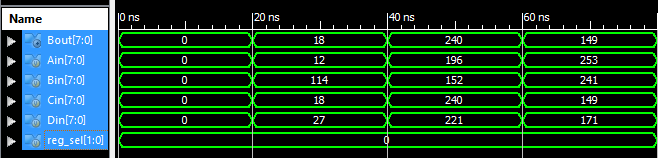
\includegraphics[width=18cm]{mux3_1.png} \\ \\
            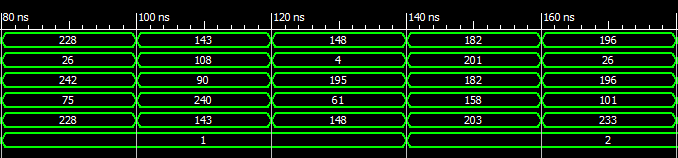
\includegraphics[width=18cm]{mux3_2.png} \\ \\
            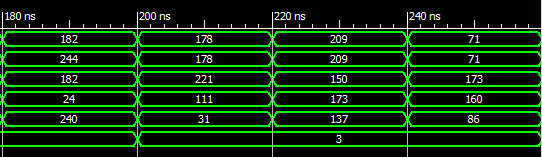
\includegraphics[width=18cm]{mux3_3.png} \\ \\
                図3 mux3のタイミングチャート
        \end{center} 

        \begin{center}
            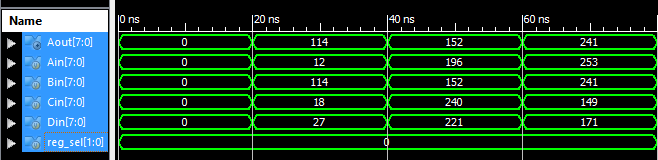
\includegraphics[width=18cm]{mux4_1.png} \\ \\
            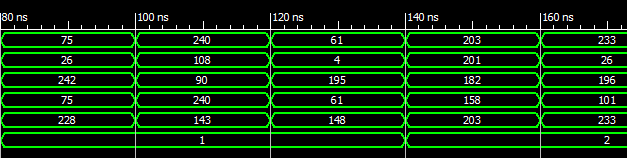
\includegraphics[width=18cm]{mux4_2.png} \\ \\
            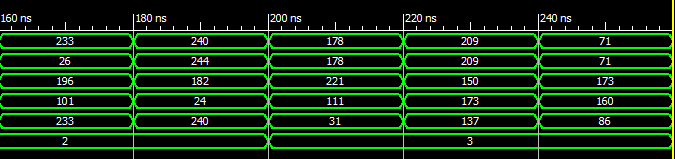
\includegraphics[width=18cm]{mux4_3.png} \\ \\
                図4 mux4のタイミングチャート
        \end{center} 
        \newpage
        図3の実行結果をまとめ, mux3の実行結果の入出力表を表4に示す. 

            \begin{table}[htb]
              \begin{center}
                \caption{mux3実行結果の入出力表}
                \begin{tabular} {|c|c|c|c|c|c|} \hline
                  \multicolumn{5}{|c|}{入力} & 出力 \\ \hline \hline
                        Ain & Bin & Cin & Din & reg\_sel & Bout \\ \hline
                        12 & 114 & 18 & 27 & 0 & 18 \\ \hline
                        196 & 152 & 240 & 221 & 0 & 240 \\ \hline
                        253 & 241 & 149 & 171 & 0 & 149 \\ \hline

                        26 & 242 & 75 & 228 & 1 & 228 \\ \hline
                        108 & 90 & 240 & 143 & 1 & 143 \\ \hline
                        4 &  195 & 61 & 148 & 1 & 148 \\ \hline

                        201 & 182 & 158 & 203 & 2 & 182 \\ \hline
                        26 & 196 & 101 & 233 & 2 & 196 \\ \hline
                        244 & 182 & 24 & 240 & 2 & 182 \\ \hline

                        178 & 221 & 111 & 31 & 3 & 178 \\ \hline
                        209 & 150 & 173 & 137 & 3 & 209 \\ \hline
                        71 & 173 & 160 & 86 & 3 & 71 \\ \hline

                \end{tabular}
              \end{center}
            \end{table}
            \newpage
            図4の実行結果をまとめ, mux4の実行結果の入出力表を表5に示す. 

            \begin{table}[htb]
              \begin{center}
                \caption{mux4実行結果の入出力表}
                \begin{tabular} {|c|c|c|c|c|c|} \hline
                  \multicolumn{5}{|c|}{入力} & 出力 \\ \hline \hline
                        Ain & Bin & Cin & Din & reg\_sel & Aout \\ \hline
                        12 & 114 & 18 & 27 & 0 & 114 \\ \hline
                        196 & 152 & 240 & 221 & 0 & 152 \\ \hline
                        253 & 241 & 149 & 171 & 0 & 241 \\ \hline

                        26 & 242 & 75 & 228 & 1 & 75 \\ \hline
                        108 & 90 & 240 & 143 & 1 & 240 \\ \hline
                        4 &  195 & 61 & 148 & 1 & 61 \\ \hline

                        201 & 182 & 158 & 203 & 2 & 203 \\ \hline
                        26 & 196 & 101 & 233 & 2 & 233 \\ \hline
                        244 & 182 & 24 & 240 & 2 & 240 \\ \hline

                        178 & 221 & 111 & 31 & 3 & 178 \\ \hline
                        209 & 150 & 173 & 137 & 3 & 209 \\ \hline
                        71 & 173 & 160 & 86 & 3 & 71 \\ \hline

                \end{tabular}
              \end{center}
            \end{table}

            ソースコード5, 6, 7, 8, 図3, 図4, 表4, 表5より, マルチプレクサー(mux3, mux4)が正しく動作していることについて説明する. 
            mux4は第1章表1のCPU命令表の1000から1010, mux3は1011から1100の範囲でAout, Boutに命令表通りにAin, Bin, Cin, Dinを出力する. ここで, Aout, Boutの出力が不定になってしまうのを避けるためにmux4ではreg\_selが11のとき, mux3ではreg\_selが10のときにAin, BinをAout, Boutにそのまま出力する. またこれにより入力する値を変える, つまり, 回路をのつなぐ端子を変えることによって, mux4はmux3の動作を, または逆にmux3をmux4の動作をすることができるため, mux4, mux3のどちらかだけでマルチプレクサーを表現することができる. 表4より, mux3はreg\_selが, 0のときはCinの値, 1のときはDinの値, 2のときはBinの値, 3のときはBinの値がAoutに出力されていることが確認することができる. 表5より, mux4はreg\_selが, 0のときはBinの値, 1のときはCinの値, 2のときはDinの値, 3のときはAinの値がAoutに出力されていることが確認することができる. これよりマルチプレクサーは正しく動作していることが確認することができる. 

    \chapter*{第5章 8bitCPU}
        cpu\_combのverilogモジュールとテストのソースコード, cpu\_comb.v, cpu\_comb\_b.v, 実行結果のタイミングチャートをソースコード9, ソースコード10, 図5に示す. 

        \begin{center}
            \begin{lstlisting}[basicstyle=\ttfamily\footnotesize, frame=single]
module cpu_comb(Ain,  Bin,  Cin,  Din,  Carryin, op,
                     Aout, Bout, Cout, Dout, Carryout);
    
    input [7:0] Ain, Bin, Cin, Din;
    input Carryin;
    input [3:0] op;
    
    output [7:0] Aout, Bout, Cout, Dout;
    output Carryout;

    wire [2:0] op_sel;
    wire [1:0] reg_sel1, reg_sel2;
    wire [7:0] alu_out;

    wire alu_enabled;

    op_decode decoder (op, op_sel, reg_sel1, reg_sel2, alu_enabled);
    alu_pp44 alu (.Ain(Ain), .Bin(Bin), .Carryin(Carryin), .op(op),
        .alu_enabled(alu_enabled), .Carryout(Carryout), .alu_out(alu_out));
    mux4 m4 (.Ain(alu_out), .Bin(Bin), .Cin(Cin), .Din(Din),
        .reg_sel(reg_sel1), .Aout(Aout));
    mux3 m3 (.Ain(alu_out), .Bin(Bin), .Cin(Cin), .Din(Din),
        .reg_sel(reg_sel2), .Bout(Bout));
    
    assign Cout = (op == 4'b1110) ? Ain : Cin;
    assign Dout = (op == 4'b1111) ? Ain : Din;
endmodule
            \end{lstlisting}
            ソースコード9 cpu\_comb.v
        \end{center}
    

        \begin{center}
            \begin{lstlisting}[basicstyle=\ttfamily\footnotesize, frame=single]
module cpu_comb_tb;

    // Inputs
    reg [7:0] Ain;
    reg [7:0] Bin;
    reg [7:0] Cin;
    reg [7:0] Din;
    reg Carryin;
    reg [3:0] op;

    // Outputs
    wire [7:0] Aout;
    wire [7:0] Bout;
    wire [7:0] Cout;
    wire [7:0] Dout;
    wire Carryout;
    
    // Instantiate the Unit Under Test (UUT)
    cpu_comb uut (
        .Ain(Ain), 
        .Bin(Bin), 
        .Cin(Cin), 
        .Din(Din), 
        .Carryin(Carryin), 
        .op(op), 
        .Aout(Aout), 
        .Bout(Bout), 
        .Cout(Cout), 
        .Dout(Dout), 
        .Carryout(Carryout)
    );

    initial begin
        // Initialize Inputs
        Ain = 0;
        Bin = 0;
        Cin = 0;
        Din = 0;
        Carryin = 0;
        op = 0;

        // Wait 100 ns for global reset to finish
        #10 Ain = 101; Bin = 58;  Cin = 83;  Din = 87;  Carryin = 0; op = 0;
        #10 Ain = 230; Bin = 37;  Cin = 242; Din = 51;  Carryin = 0; op = 0;
        #10 Ain = 153; Bin = 2;   Cin = 176; Din = 33;  Carryin = 0; op = 0;
        #10 Ain = 11;  Bin = 182; Cin = 13;  Din = 65;  Carryin = 1; op = 0;
  
        #10 Ain = 0;   Bin = 204; Cin = 228; Din = 220; Carryin = 0; op = 1;
        #10 Ain = 70;  Bin = 60;  Cin = 71;  Din = 75;  Carryin = 1; op = 1;
        #10 Ain = 151; Bin = 92;  Cin = 224; Din = 8;   Carryin = 1; op = 1;
        #10 Ain = 117; Bin = 183; Cin = 108; Din = 56;  Carryin = 0; op = 1;
  
        #10 Ain = 181; Bin = 155; Cin = 244; Din = 225; Carryin = 1; op = 2;
        #10 Ain = 188; Bin = 8;   Cin = 110; Din = 220; Carryin = 0; op = 2;
        #10 Ain = 237; Bin = 17;  Cin = 240; Din = 237; Carryin = 0; op = 2;
        #10 Ain = 179; Bin = 170; Cin = 231; Din = 210; Carryin = 1; op = 2;
  
        #10 Ain = 214; Bin = 52;  Cin = 96;  Din = 97;  Carryin = 1; op = 3;
        #10 Ain = 194; Bin = 77;  Cin = 82;  Din = 175; Carryin = 0; op = 3;
        #10 Ain = 57;  Bin = 198; Cin = 24;  Din = 124; Carryin = 0; op = 3;
        #10 Ain = 227; Bin = 86;  Cin = 185; Din = 228; Carryin = 0; op = 3;
  
        #10 Ain = 236; Bin = 182; Cin = 61;  Din = 119; Carryin = 0; op = 4;
        #10 Ain = 59;  Bin = 168; Cin = 54;  Din = 152; Carryin = 0; op = 4;
        #10 Ain = 98;  Bin = 19;  Cin = 203; Din = 180; Carryin = 0; op = 4;
        #10 Ain = 200; Bin = 250; Cin = 243; Din = 89;  Carryin = 1; op = 4;
  
        #10 Ain = 202; Bin = 173; Cin = 54;  Din = 35;  Carryin = 0; op = 5;
        #10 Ain = 39;  Bin = 23;  Cin = 91;  Din = 87;  Carryin = 1; op = 5;
        #10 Ain = 217; Bin = 74;  Cin = 152; Din = 104; Carryin = 1; op = 5;
        #10 Ain = 71;  Bin = 179; Cin = 103; Din = 174; Carryin = 1; op = 5;
  
        #10 Ain = 46;  Bin = 244; Cin = 113; Din = 230; Carryin = 1; op = 6;
        #10 Ain = 209; Bin = 49;  Cin = 50;  Din = 204; Carryin = 0; op = 6;
        #10 Ain = 96;  Bin = 225; Cin = 170; Din = 28;  Carryin = 1; op = 6;
        #10 Ain = 152; Bin = 238; Cin = 221; Din = 142; Carryin = 1; op = 6;
  
        #10 Ain = 175; Bin = 206; Cin = 201; Din = 110; Carryin = 1; op = 7;
        #10 Ain = 16;  Bin = 26;  Cin = 106; Din = 150; Carryin = 0; op = 7;
        #10 Ain = 123; Bin = 253; Cin = 186; Din = 186; Carryin = 0; op = 7;
        #10 Ain = 85;  Bin = 133; Cin = 59;  Din = 182; Carryin = 1; op = 7;
  
        #10 Ain = 122; Bin = 33;  Cin = 217; Din = 225; Carryin = 1; op = 8;
        #10 Ain = 49;  Bin = 63;  Cin = 65;  Din = 237; Carryin = 0; op = 8;
        #10 Ain = 248; Bin = 195; Cin = 36;  Din = 114; Carryin = 1; op = 8;
        #10 Ain = 155; Bin = 206; Cin = 101; Din = 189; Carryin = 0; op = 8;
  
        #10 Ain = 170; Bin = 150; Cin = 239; Din = 179; Carryin = 0; op = 9;
        #10 Ain = 229; Bin = 179; Cin = 57;  Din = 46;  Carryin = 0; op = 9;
        #10 Ain = 236; Bin = 149; Cin = 83;  Din = 99;  Carryin = 0; op = 9;
        #10 Ain = 113; Bin = 52;  Cin = 6;   Din = 119; Carryin = 1; op = 9;
  
        #10 Ain = 237; Bin = 204; Cin = 161; Din = 223; Carryin = 0; op = 10;
        #10 Ain = 24;  Bin = 181; Cin = 91;  Din = 183; Carryin = 0; op = 10;
        #10 Ain = 44;  Bin = 174; Cin = 185; Din = 45;  Carryin = 0; op = 10;
        #10 Ain = 84;  Bin = 127; Cin = 145; Din = 187; Carryin = 0; op = 10;
  
        #10 Ain = 3;   Bin = 236; Cin = 208; Din = 147; Carryin = 1; op = 11;
        #10 Ain = 90;  Bin = 194; Cin = 197; Din = 225; Carryin = 0; op = 11;
        #10 Ain = 63;  Bin = 92;  Cin = 33;  Din = 194; Carryin = 0; op = 11;
        #10 Ain = 204; Bin = 189; Cin = 203; Din = 129; Carryin = 1; op = 11;
  
        #10 Ain = 142; Bin = 192; Cin = 105; Din = 238; Carryin = 1; op = 12;
        #10 Ain = 188; Bin = 228; Cin = 142; Din = 10;  Carryin = 0; op = 12;
        #10 Ain = 50;  Bin = 35;  Cin = 171; Din = 197; Carryin = 0; op = 12;
        #10 Ain = 119; Bin = 26;  Cin = 148; Din = 47;  Carryin = 0; op = 12;
  
        #10 Ain = 13;  Bin = 181; Cin = 52;  Din = 139; Carryin = 1; op = 13;
        #10 Ain = 198; Bin = 2;   Cin = 129; Din = 86;  Carryin = 0; op = 13;
        #10 Ain = 230; Bin = 158; Cin = 157; Din = 55;  Carryin = 0; op = 13;
        #10 Ain = 233; Bin = 54;  Cin = 57;  Din = 168; Carryin = 0; op = 13;
  
        #10 Ain = 187; Bin = 149; Cin = 107; Din = 212; Carryin = 0; op = 14;
        #10 Ain = 52;  Bin = 143; Cin = 90;  Din = 29;  Carryin = 0; op = 14;
        #10 Ain = 53;  Bin = 177; Cin = 220; Din = 40;  Carryin = 0; op = 14;
        #10 Ain = 206; Bin = 85;  Cin = 238; Din = 41;  Carryin = 0; op = 14;

        #10 Ain = 23;  Bin = 76;  Cin = 32;  Din = 246; Carryin = 0; op = 15;
        #10 Ain = 248; Bin = 197; Cin = 56;  Din = 252; Carryin = 1; op = 15;
        #10 Ain = 206; Bin = 31;  Cin = 55;  Din = 115; Carryin = 0; op = 15;
        #10 Ain = 218; Bin = 235; Cin = 93;  Din = 29;  Carryin = 0; op = 15;
        
        #10 $finish;
        // Add stimulus here

    end
      
endmodule
            \end{lstlisting}
            ソースコード10 cpu\_comb\_tb.v
        \end{center}

        \begin{center}
            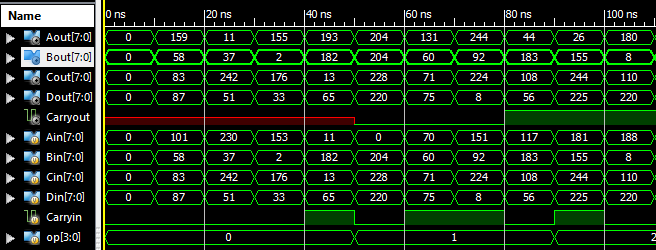
\includegraphics[width=18cm]{apu_comb_1_1.png} \\ \\
            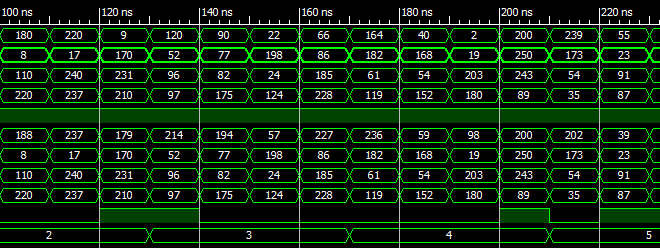
\includegraphics[width=18cm]{apu_comb_1_2.png} \\ \\
            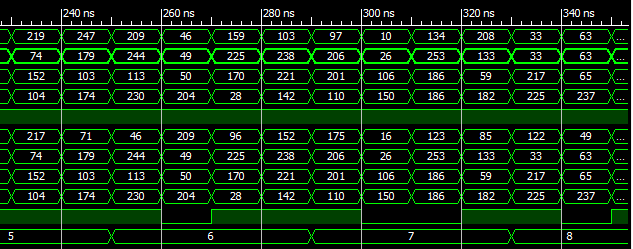
\includegraphics[width=18cm]{apu_comb_1_3.png} \\ \\

            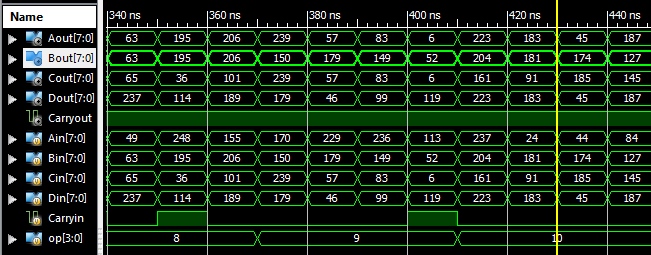
\includegraphics[width=18cm]{apu_comb_2_1.png} \\ \\
            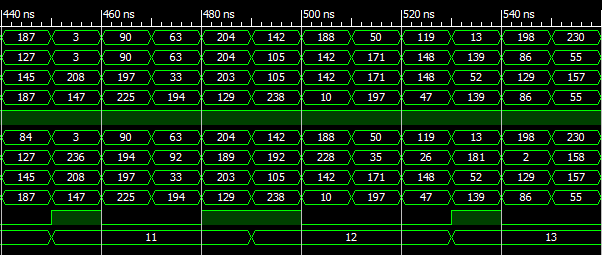
\includegraphics[width=18cm]{apu_comb_2_2.png} \\ \\ \newpage
            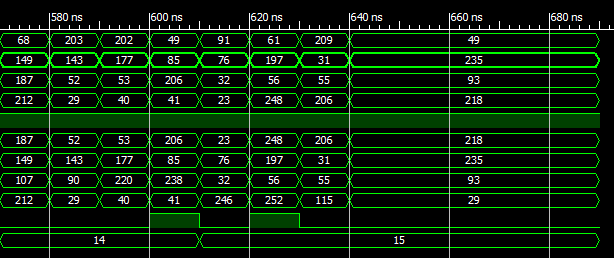
\includegraphics[width=18cm]{apu_comb_2_3.png} \\ \\
                図5 cpu\_combのタイミングチャート
        \end{center}

        図5の実行結果をまとめ, cpu\_combの実行結果の入出力表を表6に示す. 

        \begin{table}[H]
            \begin{center}
                \caption{mux4実行結果の入出力表}
                \begin{tabular} {|c|c|c|c|c|c|c|c|c|c|c|} \hline
                    \multicolumn{6}{|c|}{入力} & \multicolumn{5}{|c|}{出力} \\ \hline \hline
                    Ain & Bin & Cin & Din & Carryin & op & Aout & Bout & Cout & Dout & Carryout \\ \hline
                    101 & 58 & 83 & 87 & 0 & 0 & 159 & 58 & 83 & 87 & 不定\\ \hline
                    230 & 37 & 242 & 51 & 0 & 0 & 11 & 37 & 242 & 51 & 不定 \\ \hline
                    153 & 2 & 176 & 33 & 0 & 0 & 155 & 2 & 176 & 33 & 不定 \\ \hline
                    11 & 182 & 13 & 65 & 1 & 0 & 193 & 182 & 13 & 65 & 不定 \\ \hline

                    0 & 204 & 228 & 220 & 0 & 1 & 204 & 204 & 228 & 220 & 0 \\ \hline
                    70 & 60 & 71 & 75 & 1 & 1 & 131 & 60 & 71 & 75 & 0 \\ \hline
                    151 & 92 & 224 & 8 & 1 & 1 & 244 & 92 & 224 & 8 & 0 \\ \hline
                    117 & 183 & 108 & 56 & 0 & 1 & 44 & 183 & 108 & 56 & 1 \\ \hline

                    181 & 155 & 244 & 225 & 1 & 2 & 26 & 155 & 244 & 225 & 1 \\ \hline
                    188 & 8 & 110 & 220 & 0 & 2 & 180 & 8 & 110 & 220 & 1 \\ \hline
                    237 & 17 & 240 & 237 & 0 & 2 & 220 & 17 & 240 & 237 & 1 \\ \hline
                    179 & 170 & 231 & 210 & 1 & 2 & 9 & 170 & 231 & 210 & 1 \\ \hline

                    214 & 52 & 96 & 97 & 1 & 3 & 120 & 52 & 96 & 97 & 1 \\ \hline
                    194 & 77 & 82 & 175 & 0 & 3 & 90 & 77 & 82 & 175 & 1 \\ \hline
                    57 & 198 & 24 & 124 & 0 & 3 & 22 & 198 & 24 & 124 & 1 \\ \hline
                    227 & 86 & 185 & 228 & 0 & 3 & 66 & 86 & 185 & 228 & 1 \\ \hline

                    236 & 182 & 61 & 119 & 0 & 4 & 164 & 182 & 61 & 119 & 1 \\ \hline
                    59 & 168 & 54 & 152 & 0 & 4 & 40 & 168 & 54 & 152 & 1 \\ \hline
                    98 & 19 & 203 & 180 & 0 & 4 & 2 & 19 & 203 & 180 & 1 \\ \hline
                    200 & 250 & 243 & 89 & 1 & 4 & 200 & 250 & 243 & 89 & 1 \\ \hline

                    202 & 173 & 54 & 35 & 0 & 5 & 239 & 173 & 54 & 35 & 1 \\ \hline
                    39 & 23 & 91 & 87 & 1 & 5 & 55 & 23 & 91 & 87 & 1 \\ \hline
                    217 & 74 & 152 & 104 & 1 & 5 & 219 & 74 & 152 & 104 & 1 \\ \hline
                    71 & 179 & 103 & 174 & 1 & 5 & 247 & 179 & 103 & 174 & 1 \\ \hline

                    46 & 244 & 113 & 230 & 1 & 6 & 209 & 244 & 113 & 230 & 1 \\ \hline
                    209 & 49 & 50 & 204 & 0 & 6 & 46 & 49 & 50 & 204 & 1 \\ \hline
                    96 & 225 & 170 & 28 & 1 & 6 & 159 & 225 & 170 & 28 & 1 \\ \hline
                    152 & 238 & 221 & 142 & 1 & 6 & 103 & 238 & 221 & 142 & 1 \\ \hline

                    175 & 206 & 201 & 110 & 1 & 7 & 97 & 206 & 201 & 110 & 1 \\ \hline
                    16 & 26 & 106 & 150 & 0 & 7 & 10 & 26 & 106 & 150 & 1 \\ \hline
                    123 & 253 & 186 & 186 & 0 & 7 & 134 & 253 & 186 & 186 & 1 \\ \hline
                    85 & 133 & 59 & 182 & 1 & 7 & 208 & 133 & 59 & 182 & 1 \\ \hline

                    122 & 33 & 217 & 225 & 1 & 8 & 33 & 33 & 217 & 225 & 1 \\ \hline
                    49 & 63 & 65 & 237 & 0 & 8 & 63 & 63 & 65 & 237 & 1 \\ \hline
                    248 & 195 & 36 & 114 & 1 & 8 & 159 & 195 & 36 & 114 & 1 \\ \hline
                    155 & 206 & 101 & 189 & 0 & 8 & 206 & 206 & 101 & 189 & 1 \\ \hline

                    170 & 150 & 239 & 179 & 0 & 9 & 239 & 150 & 239 & 179 & 1 \\ \hline
                    229 & 179 & 57 & 46 & 0 & 9 & 57 & 179 & 57 & 46  & 1 \\ \hline
                \end{tabular} \newpage
            \end{center}
        \end{table}
        \begin{table}[H]
            \begin{center}
                \begin{tabular} {|c|c|c|c|c|c|c|c|c|c|c|} \hline
                    \multicolumn{6}{|c|}{入力} & \multicolumn{5}{|c|}{出力} \\ \hline \hline
                    Ain & Bin & Cin & Din & Carryin & op & Aout & Bout & Cout & Dout & Carryout \\ \hline
                    236 & 149 & 83 & 99 & 0 & 9 & 83 & 149 & 83 & 99  & 1 \\ \hline
                    113 & 52 & 6 & 119 & 1 & 9 & 6 & 52 & 6 & 119 & 1 \\ \hline

                    237 & 204 & 161 & 223 & 0 & 10 & 223 & 204 & 161 & 223  & 1 \\ \hline
                    24 & 181 & 91 & 183 & 0 & 10 & 183 & 181 & 91 & 183 & 1 \\ \hline
                    44 & 174 & 185 & 45 & 0 & 10 & 45 & 174 & 185 & 45 & 1 \\ \hline
                    84 & 127 & 145 & 187 & 0 & 10 & 187 & 127 & 145 & 187 & 1 \\ \hline

                    3 & 236 & 208 & 147 & 1 & 11 & 3 & 3 & 208 & 147 & 1 \\ \hline
                    90 & 194 & 197 & 225 & 0 & 11 & 90 & 90 & 197 & 225 & 1 \\ \hline
                    63 & 92 & 33 & 194 & 0 & 11 & 63 & 63 & 33 & 194 & 1 \\ \hline
                    204 & 189 & 203 & 129 & 1 & 11 & 204 & 204 & 203 & 129 & 1 \\ \hline

                    142 & 192 & 105 & 238 & 1 & 12 & 142 & 105 & 105 & 238 & 1 \\ \hline
                    188 & 228 & 142 & 10 & 0 & 12 & 188 & 142 & 142 & 10 & 1 \\ \hline
                    50 & 35 & 171 & 197 & 0 & 12 & 50 & 171 & 171 & 197 & 1 \\ \hline
                    119 & 26 & 148 & 47 & 0 & 12 & 119 & 148 & 148 & 47 & 1 \\ \hline

                    13 & 181 & 52 & 139 & 1 & 13 & 13 & 139 & 52 & 139 & 1 \\ \hline
                    198 & 2 & 129 & 86 & 0 & 13 & 198 & 86 & 129 & 86 & 1 \\ \hline
                    230 & 158 & 157 & 55 & 0 & 13 & 230 & 55 & 157 & 55 & 1 \\ \hline
                    233 & 54 & 57 & 168 & 0 & 13 & 233 & 54 & 57 & 168 & 1 \\ \hline

                    187 & 149 & 107 & 212 & 0 & 14 & 187 & 149 & 187 & 212 & 1 \\ \hline
                    52 & 143 & 90 & 29 & 0 & 14 & 52 & 143 & 52 & 29 & 1 \\ \hline
                    53 & 177 & 220 & 40 & 0 & 14 & 53 & 177 & 53 & 40 & 1 \\ \hline
                    206 & 85 & 238 & 41 & 0 & 14 & 206 & 85 & 206 & 41 & 1 \\ \hline

                    23 & 76 & 32 & 246 & 0 & 15 & 23 & 76 & 32 & 23 & 1 \\ \hline
                    248 & 197 & 56 & 252 & 1 & 15 & 248 & 197 & 56 & 248 & 1 \\ \hline
                    206 & 31 & 55 & 115 & 0 & 15 & 206 & 31 & 55 & 206 & 1 \\ \hline
                    218 & 235 & 93 & 29 & 0 & 15 & 218 & 235 & 93 & 218 & 1 \\ \hline
                \end{tabular}
            \end{center}
        \end{table}

        ソースコード9, 10, 図5, 表6,より, 8bitCPU(cpu\_comb)が正しく動作していることについて説明する. まず, 演算命令の部分は以下の式が成り立つことによりAoutに演算結果が出力されていることが確認することができる. また, Aout以外の出力端子は, Bout, Cout, Doutには, Bin, Cin, Dinをそのまま出力し, CarryoutにはADC命令以外は前の出力をそのまま出力し, ADC命令時にはキャリーならHighが出力されていることが確認できる. また, 転送命令は, 命令(op)が1000のときAoutにBinを, 命令(op)が1001のときAoutにCinを, 命令(op)が1010のときAoutにDinを, 命令(op)が1011のときBoutにAinを, 命令(op)が1100のときBoutにCinを, 命令(op)が1101のときBoutにDinを, 命令(op)が1110のときCoutにAinを, 命令(op)が1111のときDoutにAinを出力し, 出力に影響しない出力端子は同じレジスタの入力端子をそのまま出力していることが確認できるので8bitCPUが正しく動作していることが分かる. 

        \begin{eqnarray*}
            Aout &=& 101 + 58 = 159 \\
            Aout &=& 230 + 37 = 11100110 + 100101 = 11 \\
            Aout &=& 153 + 2 = 155 \\
            Aout &=& 11 + 182 = 193 \\
            Aout &=& 0 + 204 = 204 \\
            Aout &=& 70 + 60 + 1 = 131 \\
            Aout &=& 151 + 92 + 1 = 244 \\
            Aout &=& 117 + 183 = 1110101 + 10110111 = 100101100 = 44 \\
            Aout &=& 181 - 155 = 26 \\
            Aout &=& 188 - 8 = 180 \\
            Aout &=& 237 - 17 = 220 \\
            Aout &=& 179 - 170 = 9 \\
            Aout &=& 214 * 52 = 11010110 * 110100 = (101011)01111000 = 120 \\
            Aout &=& 194 * 77 = 11000010 * 1001101 = (111010)01011010 = 90 \\
            Aout &=& 57 * 198 = 111001 * 11000110 = (101100)00010110 = 22 \\
            Aout &=& 227 * 86 = 11100011 * 1010110 = (1001100)01000010 = 66 \\
            Aout &=& 236 and 182 = 11101100 \wedge 10110110 = 10100100 = 164 \\
            Aout &=& 59 and 168 = 111011 \wedge 10101000 = 101000 = 40 \\
            Aout &=& 98 and 19 = 1100010 \wedge 10011 = 10 = 2 \\
            Aout &=& 200 and 250 = 11001000 \wedge 11111010 = 11001000 = 200 \\
            Aout &=& 202 or 173 = 11001010 \vee 10101101 = 11101111 = 239 \\
            Aout &=& 39 or 23 = 100111 \vee 10111 = 55 \\
            Aout &=& 217 or 74 = 11011001 \vee 1001010 = 11011011 = 219 \\
            Aout &=& 71 or 179 = 1000111 \vee 10110011 = 11110111 = 247 \\
            Aout &=& not 46 = \overline{101110} = 11010001 \\
            Aout &=& not 209 = \overline{11010001} = 10011111 \\
            Aout &=& not 96 = \overline{1100000} = 1100111 \\
            Aout &=& not 152 = \overline{10011000} = 1100001 \\
            Aout &=& 175 xor 206 = 10101111 \oplus 11001110 = 1100001 = 97 \\
            Aout &=& 16 xor 26 = 10000 \oplus 11010 = 1010 = 10 \\
            Aout &=& 123 xor 253 = 1111011 \oplus 11111101 = 10000110 = 134 \\
            Aout &=& 85 xor 133 = 1010101 \oplus 10000101 = 11010000 = 208 \\
        \end{eqnarray*}

        ソースコード11にmux3の代わりにmux4を使ったcpu\_combの修正部分のソースコードを示す. mux3とmux4は端子をつなぎかえることによってお互い代替可能なので, どちらか片方のモジュールを使いまわすほうが, 修正が効きやすく部品の種類が減り, 結果的にコストダウンにつながる. 
         \begin{center}
            \begin{lstlisting}[basicstyle=\ttfamily\footnotesize, frame=single]
        // mux3 m3 (.Ain(alu_out), .Bin(Bin), .Cin(Cin), .Din(Din),
            .reg_sel(reg_sel2), .Bout(Bout));
        mux4 m3 (.Ain(alu_out), .Bin(Cin), .Cin(Din), .Din(Bin),
            .reg_sel(reg_sel2), .Aout(Bout));
            \end{lstlisting}
            ソースコード11 mux3の代わりにmux4を使ったcpu\_comb.vの修正部
        \end{center}
        完成した8bitCPUのブロック図を図6に示す. また、このブロック図はmux3を使用しておらず、mux3の動作を繋ぐ端子を変えることにより、mux4が行っている。
        \begin{center}
            \includegraphics[width=18cm]{Untitled_Diagram.png} \\ \\
                図6 cpu\_combのブロック図
        \end{center}
\end{document}
